\documentclass[a4paper]{scrreprt}

\usepackage[german]{babel}
\usepackage[utf8]{inputenc}
\usepackage[T1]{fontenc}
\usepackage{ae}
\usepackage{amssymb}
\usepackage{graphicx}
\usepackage{hyperref}

\begin{document}

\title{BS Zusammenfassung}
\author{Benedict Hauck, Fedor Scholz}
\maketitle

\tableofcontents
\vspace{1cm}

\chapter{01aIntro}

\section{Was ist ein Betriebssystem?}

\begin{itemize}
	\item Vermittler zwischen Benutzer und Computer
	\item Ziele
		\begin{itemize}
			\item Benutzerprogramme ausfuehren und dem Benutzer das Loesen von Problemen erleichtern
			\item Computer benutzbarer machen
			\item Hardware des Computer effizient nutzen
		\end{itemize}
	\item Vier Komponenten eines Computersystems
		\begin{itemize}
			\item Benutzer
			\item System- und Anwendungsprogramme
			\item Betriebssystem
			\item Hardware
		\end{itemize}
	\item Betriebssysteme verteilen Ressourcen
		\begin{itemize}
			\item Verwaltung aller Ressourcen
			\item Entscheidung bei konfligierenden Anfragen fuer effizientes und faires Benutzen der Ressourcen
		\end{itemize}
	\item Betriebssysteme kontrollieren
		\begin{itemize}
			\item Kontrolle von Ausfuehrungen von Programmen um Fehler und ungeeignetes Benutzen des Computers zu verhindern
		\end{itemize}
	\item Das Programm, welches immer laeuft, ist der Kernel. Alles andere ist entweder ein System- oder Anwendungsprogramm
	\item Das bootstrap program wird beim Starten oder Neustarten geladen
		\begin{itemize}
			\item Wird in ROM, EPROM oder FLASH als firmware gespeichert
			\item Initialisiert alle Aspekte des Systems, insbesondere die HW-Komponenten
			\item Laedt den Kernel und startet die Ausfuehrung
		\end{itemize}
\end{itemize}

\section{Organisation}

\begin{itemize}
	\item Ein oder mehr CPUs, device controllers verbinden sich ueber den Bus um Zugriff auf shared memory zu bekommen
	\item I/O-Geraete und CPU koennen gleichzeitig ausfuehren
	\item Jeder device controller ist zustaendig fuer einen Geraetetypen
	\item Jeder device controller hat einen lokalen Puffer
	\item CPU bewegt Daten vom/zum Hauptspeicher zu/von lokalen Puffern
	\item I/O ist vom Geraet zum lokalen Puffer des controllers
	\item device controller informiert CPU per interrupts, wenn er fertig ist
\end{itemize}


\section{Interrupts}

\subsection{Haeufige Funktionen von Interrupts}

\begin{itemize}
	\item interrupt gibt Kontrolle an interrupt service routine ueber einen interrupt vector, welcher die Adressen von allen service routines beinhaltet
	\item interrupt architecture muss Adresse der unterbrochenen Intruktion speichern
	\item Einkommende interrupts sind aus, wenn gerade ein anderer bearbeitet wird um lost interrupts zu verhindern
	\item trap ist ein interrupt, welcher von Software verursacht wurde (wegen eines Fehler oder durch eine Benutzeranfrage)
	\item Betriebssysteme sind interrupt driven
\end{itemize}

\subsection{Timer interrupts}

\begin{itemize}
	\item Time interrupts um endlose Schleifen und Prozesse zu verhindern
	\item Wird nach bestimmter Zeitspanne ausgefuehrt
	\item Wird vor dem schedulen des Programm aufgesetzt
	\item Eingebettete Systeme haben Watchdog, welche bis 0 zaehlt und dann resettet
\end{itemize}

\subsection{Interrupt Handling}

\begin{itemize}
	\item Betriebssystem merkt sich Status der CPU, indem es Register und Programmzaehler speichert
	\item Legt Typ des interrupts fest
		\begin{itemize}
			\item polling
			\item vectored interrupt system
		\end{itemize}
\end{itemize}

\section{I/O Struktur}

\subsection{Synchrone oder blockende I/O}

\begin{itemize}
	\item Nachdem I/O beginnt, geht die Kontrolle erst nach Fertigstellung der I/O wieder zum Benutzerprogramm
	\item Wait instruction laesst die CPU idlen
	\item Meistens nur ein I/O Request gleichzeitig
	\item Polling
	\item Signal
	\item Callback function
\end{itemize}

\subsection{Direct Memory Access Structure}

\begin{itemize}
	\item Fuer high-speed I/O, damit diese mit fast der Geschwindigkeit des Hauptspeichers Informationen uebertragen koennen
	\item Device Controller uebertraegt Daten in Bloecken vom Puffer direkt in den Hauptspeicher ohne CPU Eingriff
	\item Nur ein interrupt pro Block
\end{itemize}

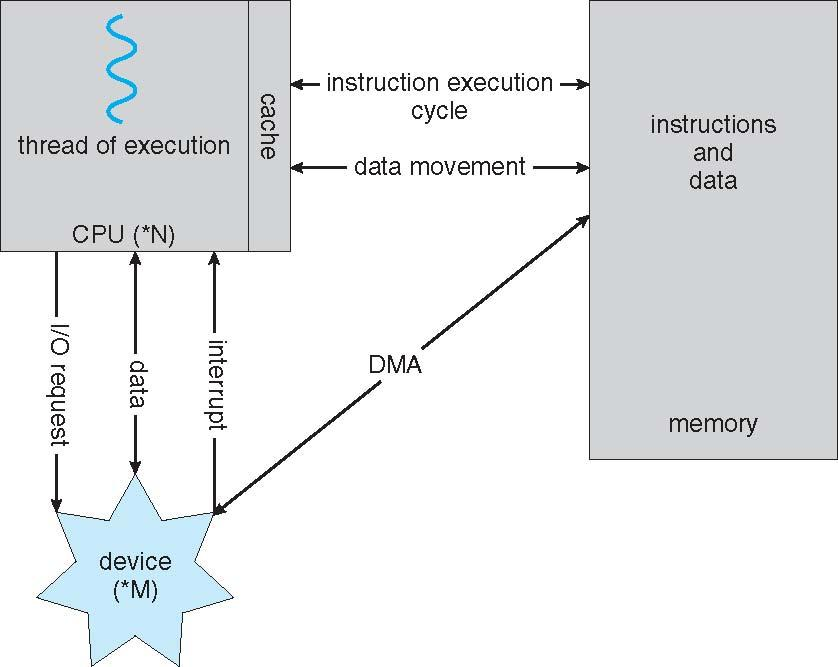
\includegraphics[scale=0.4]{dma.png}









\chapter{01bCProgramming}
\chapter{02OS}

\section{Monolithisches System}
Vorteile:
	\begin{itemize} 
		\item Einfacher Zugriff auf alle Systemdaten 
		\item Kosten von Modulinteraktionen sind niedrig
		\item Erweiterbar über Schnittstellen
		\item Vorhersehbares Verhalten 
	\end{itemize}
Nachteile:
	\begin{itemize}
		\item Kein Schutz zwischen System und Anwendung
		\item Instabil
	\end{itemize}

Beispiele:
	\begin{itemize}
		\item uCLinux, RTOSe, eCos
	\end{itemize}
	
\section{Mehrschichtiger Ansatz}
	\begin{itemize}
		\item Betriebssystem ist in n Schichten aufgeteilt
		\item Jede Schicht kann nur auf die Funktionen und Dienste von niedrigeren Schichten zugreifen 
			\begin{itemize} 
				\item Schicht 0 ist die Hardware
				\item Schicht n ist das Benutzerinterface
			\end{itemize}
		\item Einfachere Migration zwischen Plattformen
		\item Einfachere Evolution der Hardwareplattform
		\item Niedrigere Schichten implementieren Mechanismen
		\item Höhere Schichten implementieren meistens Policies
	\end{itemize}

\begin{center}
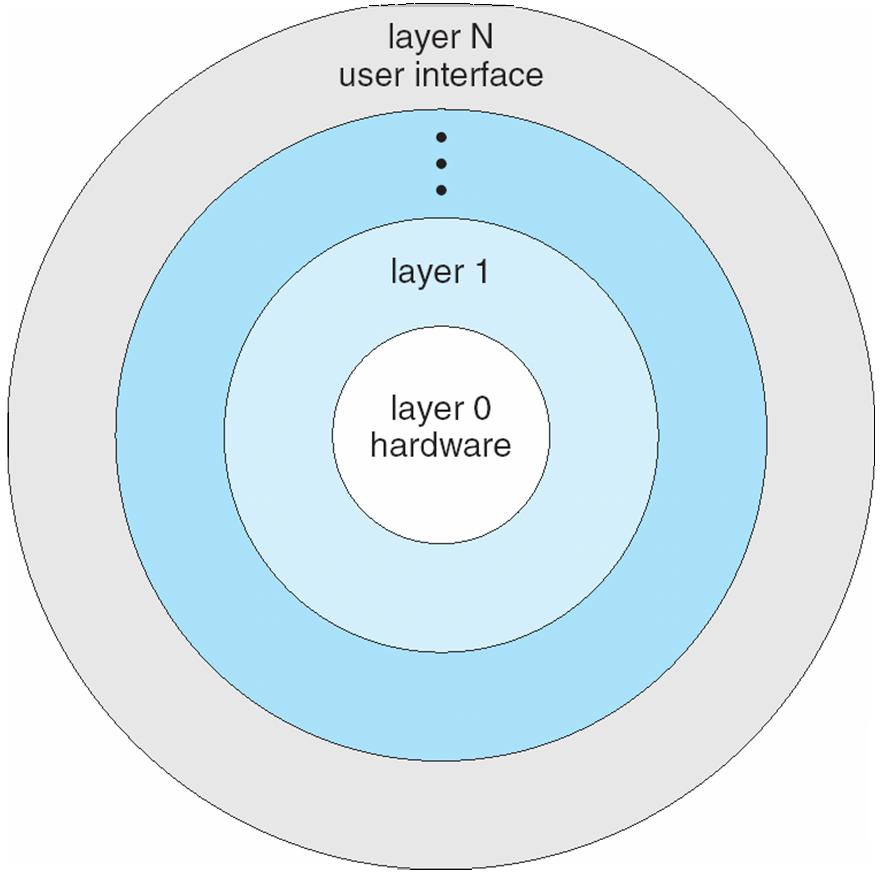
\includegraphics[scale=0.15] {schichtenmodell.png} 
\end{center}

Vorteile:
	\begin{itemize}
		\item Jede Schicht kann unabhängig getestet und verfiziert werden
		\item Korrektheit von Schicht n hängt nur von Schicht n-1 ab (einfacheres Debugging, einfachere Wartung)
	\end{itemize}

Nachteile:
	\begin{itemize}
		\item Nur unidirektionaler Schutz
		\item Beiseitige Abhängigkeit von Schichten verhindert strikte Schichtenbildung
	\end{itemize}
Beispiele:
	\begin{itemize}
		\item THE (Dijkstra), Multics(GE), VOCOS(EWSD)
	\end{itemize}

\chapter{03aProcess-management}
\chapter{03bProcess-management-scheduling}
\chapter{04Process-coordination}
\chapter{05aMemoryManagement}
\chapter{05bMemoryManagement}
\chapter{05cMemoryManagement}
\chapter{06aFileSystems}
\chapter{06bFileSystems}
\chapter{07aImplementingFileSystems}
\chapter{07bImplementingFileSystems}
\chapter{08SecondaryStorageStructure}
\chapter{09IoSystems}

\end{document}
